\documentclass[journal]{IEEEtran}
\usepackage[T1]{fontenc}
\usepackage{cite}
\usepackage{amsmath,amssymb,amsfonts}
\usepackage{graphicx}
\usepackage{textcomp}
\usepackage{booktabs}
\usepackage{array}
\usepackage{algorithm}
\usepackage{algpseudocode}
\usepackage{url}
\usepackage{microtype}
\hyphenation{op-tical net-works semi-conduc-tor IEEE-Xplore Ben-ja-mi-ni Hoch-berg Bon-fer-ro-ni}

\begin{document}

\title{Scaling ML Observability from Pilot to Portfolio: Measured Drift-Detector Behavior and False-Alarm Control for Hundreds of Models}

\author{Bhavin~Kotak%
\thanks{B. Kotak is with IBM, Armonk, NY, USA (e-mail: bhavin.kotak@ibm.com; ORCID: 0009-0006-4793-7046).}%
\thanks{Version 2.0. This revision replaces the unmeasured quantitative claims of version 1 with experiments whose code, data, and logged results are archived with the paper.}}

\markboth{Preprint, version 2.0}%
{Kotak: Scaling ML Observability from Pilot to Portfolio}

\maketitle

\begin{abstract}
Version 1 of this paper proposed a way to scale machine learning observability from one model to a portfolio, but its quantitative claims could not be traced to data or code. This revision replaces them with measurements. We benchmark five univariate drift detectors (population stability index, Kullback-Leibler divergence, binned chi-square, Kolmogorov-Smirnov, and Wasserstein-1) on 27 features from three public datasets with injected drift. We also simulate portfolios of up to 1000 models with 20 monitored features each, and on the real Elec2 electricity stream we compare input-drift alarms with performance alarms. Drift in the first two studies is simulated. A rule-of-thumb threshold does not fix a false alarm rate: the PSI rule fired on 22.1\% of no-drift numeric windows of 100 rows and on none of 2000 rows. Once every detector was calibrated to the same false alarm rate, none was best for all drift types. In the simulated portfolio of 1000 models, per-test thresholds raised 956.4 false feature alarms per day. The Benjamini-Hochberg procedure removed 99.6\% of them and kept 86.6\% of the per-test three-day event recall, so our preregistered hypothesis is supported. With 100-row windows, though, its three-day recall fell to 0.580. On Elec2, input-drift tests fired in all 200 monitored weeks and performance alarms in 138. Input drift was useful there for triage but could not stand in for a measure of accuracy. Code, data provenance, and logged results are archived with the paper.
\end{abstract}

\begin{IEEEkeywords}
concept drift, dataset shift, drift detection, false discovery rate, multiple testing, model monitoring, MLOps, population stability index
\end{IEEEkeywords}

\IEEEpeerreviewmaketitle

\section{Introduction}
\label{sec:intro}

\IEEEPARstart{M}{odels} in production can lose accuracy while their code stays the same. Their inputs move away from the training distribution, or the relation between inputs and labels changes~\cite{gama2014,lu2019,moreno2012}. Monitoring tools therefore compare each production feature against a reference sample and raise an alarm when a distance or a test statistic crosses a threshold~\cite{evidently,alibidetect,nannyml,klaise2020}. In interview studies and case surveys of production machine learning, monitoring comes up again and again as a hard problem~\cite{shankar2022,paleyes2022,amershi2019}.

Version 1 of this paper described a three-tier monitoring architecture and a portfolio strategy for hundreds of models. It also reported detector accuracies and reductions in detection time and alert fatigue, all taken from production case studies. None of those numbers can be traced to data, code, or logs. This revision keeps the architecture, but only as a design description. Each quantitative claim is either gone or replaced with a measurement that the archived code reproduces.

Once a team moves from one monitored model to many, two practical questions are still open. The first is about thresholds. The usual rules of thumb, such as PSI above 0.1, carry no stated false alarm rate, and how they behave depends on the window size. The second is about scale: a portfolio of $N$ models with $F$ features each runs $NF$ tests per monitoring period, so with a per-test level $\alpha$ the expected number of false alarms grows linearly in $NF$. Multiple-testing procedures address exactly this~\cite{dunn1961,benjamini1995,benjamini2001}. We are not aware of any measurement of what they cost in missed drift on drift-monitoring workloads.

We study five research questions.
\begin{itemize}[\IEEEsetlabelwidth{RQ5:}]
\item[RQ1:] How often do common threshold rules fire on windows without drift, and how does that change with window size?
\item[RQ2:] With every detector calibrated to the same false alarm rate, which one best detects which kind of injected drift on real feature distributions?
\item[RQ3:] How fast do the detectors react to gradual drift, and what does one call cost?
\item[RQ4:] At portfolio scale, how do per-test, Bonferroni, Benjamini-Hochberg (BH), and hierarchical alarm policies trade false alarms against missed drift events?
\item[RQ5:] On a real temporal stream, do input-drift alarms agree with performance-drop alarms?
\end{itemize}

The paper makes four contributions. (i) Section~\ref{sec:method} gives a formal system model of portfolio drift monitoring, with explicit outcome handling for missing data, abstentions, and timeouts. (ii) A preregistered portfolio experiment on simulated drift measures false alarms per day and three-day event recall under four alarm policies, for up to 1000 models. (iii) A calibrated benchmark compares five univariate detectors on 27 features from three public datasets with injected drift and reports the false alarm rates of rule-of-thumb thresholds. (iv) On the Elec2 stream~\cite{elec2}, we measure how well input-drift alarms agree with performance alarms. All drift in (ii) and (iii) is simulated; only (iv) uses a real shift.

\section{Related Work}
\label{sec:related}

\subsection{Drift and dataset shift}

Surveys define concept drift as a change in the joint distribution of inputs and labels, and they separate it from covariate shift and prior shift~\cite{gama2014,lu2019,webb2016,moreno2012,zliobaite2010}. Covariate shift and its correction by importance weighting go back to Shimodaira~\cite{shimodaira2000}. Label shift can be detected and corrected with black-box predictors~\cite{lipton2018}. Rabanser et al.~\cite{rabanser2019} compared shift detectors on image data, among them univariate tests with Bonferroni aggregation over dimensions and kernel two-sample tests~\cite{gretton2008}. Our unit of analysis is different. We look at many independent models with tabular features, each one monitored over and over in time.

\subsection{Univariate statistics}

The Kolmogorov-Smirnov (KS) test~\cite{massey1951}, the Kullback-Leibler divergence~\cite{kullback1951}, and the Wasserstein distance~\cite{ramdas2017} are standard two-sample summaries. The population stability index (PSI) is common in credit risk. Yurdakul and Naranjo~\cite{yurdakul2020} studied its sampling distribution, and their result is why we check fixed PSI thresholds across window sizes.

\subsection{Sequential detectors}

CUSUM and Page-Hinkley tests~\cite{page1954}, the drift detection method (DDM)~\cite{gama2004}, and ADWIN~\cite{bifet2007} monitor a stream of errors or values and adapt the window. Each targets a single stream. We do not benchmark them here, and we list that omission as a threat to validity.

\subsection{Multiple testing}

Bonferroni control~\cite{dunn1961} bounds the family-wise error rate. The BH procedure~\cite{benjamini1995} controls the false discovery rate (FDR) under independence, and Benjamini and Yekutieli~\cite{benjamini2001} showed that it also does so under positive regression dependence. Storey~\cite{storey2002} estimates the null proportion to gain power. Online FDR rules~\cite{javanmard2018,ramdas2017online} control error over a stream of tests. We evaluate the offline per-period procedures, because batch monitoring jobs run one period at a time.

\subsection{Production ML practice}

Platform papers describe data validation and monitoring as part of the ML lifecycle~\cite{baylor2017,polyzotis2018,schelter2018,breck2017}. Open-source tools implement drift tests and performance estimation without labels~\cite{evidently,alibidetect,nannyml}, and Garg et al.~\cite{garg2022} predict accuracy under shift from unlabeled data. We cite these tools for context only and attribute no measurements to them.

\section{Methodology}
\label{sec:method}

\subsection{System model}

A portfolio contains models $i\in\{1,\dots,N\}$. Model $i$ monitors features $j\in\{1,\dots,F\}$. For each pair $(i,j)$ a reference sample $\mathcal{R}_{ij}$ of size $m$ is stored at training time. In monitoring period $t\in\{1,\dots,T\}$, the system receives a window $\mathcal{W}_{ijt}$ of $n$ values. The null hypothesis of no drift is
\begin{equation}
H^{0}_{ijt}:\; P_{ijt} = P^{\mathrm{ref}}_{ij}, \qquad \theta_{ijt} = \mathbf{1}\!\left[P_{ijt}\neq P^{\mathrm{ref}}_{ij}\right],
\label{eq:system}
\end{equation}
where $P_{ijt}$ is the distribution that generated the window, $P^{\mathrm{ref}}_{ij}$ generated the reference, and $\theta_{ijt}$ is the unobserved drift indicator. A detector maps $(\mathcal{R}_{ij},\mathcal{W}_{ijt})$ to a score $s_{ijt}$ (larger means more drift) and, for tests, to a $p$-value $p_{ijt}$. An alarm policy maps the scores of one period to a set of rejected pairs. A drift event $e$ is a model $i_e$ whose features drift from onset $t_e$ onward. Every experiment below tests instances of \eqref{eq:system}. The truth $\theta_{ijt}$ is known only where we simulated the drift.

\subsection{Detectors}

Let $\hat{G}_m$ and $\hat{F}_n$ be the empirical distribution functions of the reference and the window. For numeric features, the binned detectors use the interior edges $\hat{G}_m^{-1}(b/B)$, $b=1,\dots,B-1$, with duplicates merged when the feature has ties, giving $B'\le B$ right-closed bins. For categorical features, the bins are the reference categories plus one out-of-vocabulary bin. With reference counts $r_b$, window counts $c_b$, and additive smoothing $a$,
\begin{equation}
\tilde{r}_b=\frac{r_b+a}{m+aB'},\qquad \tilde{c}_b=\frac{c_b+a}{n+aB'}.
\label{eq:smooth}
\end{equation}
We use $B=10$ and $a=0.5$. With the smoothed proportions of \eqref{eq:smooth}, the PSI and the Kullback-Leibler divergence of the window from the reference are
\begin{equation}
\mathrm{PSI}=\sum_{b=1}^{B'}(\tilde{c}_b-\tilde{r}_b)\ln\frac{\tilde{c}_b}{\tilde{r}_b},
\label{eq:psi}
\end{equation}
\begin{equation}
\mathrm{KL}=\sum_{b=1}^{B'}\tilde{c}_b\ln\frac{\tilde{c}_b}{\tilde{r}_b}.
\label{eq:kl}
\end{equation}
The binned chi-square detector applies Pearson's test to the $2\times B''$ table of raw counts, where $B''$ counts the bins with at least one observation; its score is $-\log_{10}p$. The last two detectors work directly on the empirical distribution functions:
\begin{equation}
D=\sup_x\left|\hat{F}_n(x)-\hat{G}_m(x)\right|,
\label{eq:ks}
\end{equation}
\begin{equation}
W_1=\frac{1}{\sigma_{\mathrm{ref}}}\int\left|\hat{F}_n(x)-\hat{G}_m(x)\right|dx,
\label{eq:w1}
\end{equation}
where $\sigma_{\mathrm{ref}}$ is the reference standard deviation. $D$ in \eqref{eq:ks} is the two-sample KS statistic; its $p$-value uses the Kolmogorov distribution with effective size $\mathrm{round}(nm/(n+m))$, as in SciPy's asymptotic mode~\cite{virtanen2020}. Our implementation evaluates both functions in \eqref{eq:ks} and \eqref{eq:w1} at every pooled sample point, which makes it exact with ties, and unit tests check it against SciPy. PSI \eqref{eq:psi} is the symmetrized form of KL \eqref{eq:kl}.

We call a threshold \emph{calibrated} when it is the $(1-\phi)$ quantile of the detector's scores on no-drift calibration windows for the same feature and window size. Here $\phi=0.05$. The false alarm rate is then estimated on a separate set of no-drift evaluation windows.

\subsection{Alarm policies}

Let $\mathcal{K}_t$ be the set of pairs whose test returned a $p$-value in period $t$, with $K_t=|\mathcal{K}_t|$, and let $p_{(1)}\le\dots\le p_{(K_t)}$ be the sorted $p$-values. The four policies reject $H^0_{ijt}$ as follows:
\begin{equation}
\begin{array}{@{}l@{\;\;}l@{}}
\text{per-test:} & p_{ijt}\le\alpha,\\
\text{Bonferroni:} & p_{ijt}\le\alpha/K_t,\\
\text{BH:} & p_{ijt}\le p_{(k^\ast)},\\
 & k^\ast=\max\{k: p_{(k)}\le kq/K_t\}.
\end{array}
\label{eq:policies}
\end{equation}
The hierarchical policy first combines the features within each model, then controls the FDR across models:
\begin{equation}
\pi_{it}=\min\!\Big(1,\;F_{it}\min_{j}p_{ijt}\Big),
\label{eq:hier}
\end{equation}
where $F_{it}$ is the number of available features of model $i$. BH at level $q$ is applied to $\{\pi_{it}\}_i$. A rejected model raises one alarm, and that alarm names the feature with the smallest $p$-value. We use $\alpha=q=0.05$.

\subsection{Operator objective}

Let $\mathrm{FA}_t=\sum_{(i,j)\in\mathcal{K}_t}\mathbf{1}[\text{reject}\wedge\theta_{ijt}=0]$ be the false feature alarms in period $t$, and let $\tau_e$ be the first period in which a drifted feature of event $e$ is rejected. An operator wants few late detections and has a budget $\beta$ for false alarms:
\begin{equation}
\min_{\text{policy}}\;\mathbb{E}\Big[\sum_e\mathbf{1}\left[\tau_e-t_e\ge L\right]\Big]
\quad\text{s.t.}\quad \mathbb{E}[\mathrm{FA}_t]\le\beta .
\label{eq:objective}
\end{equation}
We do not solve \eqref{eq:objective}. Instead we measure where each fixed policy lands on its two terms, with $L=3$ periods. The primary endpoints of the preregistered hypothesis compare BH with the per-test baseline:
\begin{equation}
R_{\mathrm{FA}}=1-\frac{\overline{\mathrm{FA}}_{\mathrm{BH}}}{\overline{\mathrm{FA}}_{\text{per-test}}},\qquad
RR=\frac{\mathrm{recall}_{3,\mathrm{BH}}}{\mathrm{recall}_{3,\text{per-test}}},
\label{eq:endpoints}
\end{equation}
where $\overline{\mathrm{FA}}$ is the mean of $\mathrm{FA}_t$ over periods and $\mathrm{recall}_3$ is the fraction of events with $\tau_e-t_e<3$. Under the hierarchical policy, an event counts as detected only if the named feature is one of the drifted ones.

\subsection{Outcome handling}

Each external decision procedure has a defined behavior for missing data, unknown results, and timeouts.
\begin{itemize}
\item \emph{Missing values in a window} are dropped. Their rate is reported with the result, so a pipeline that starts emitting nulls shows up even when the remaining values look stable.
\item \emph{Too few values}: a window with fewer than 30 usable values abstains with status \texttt{insufficient\_data}.
\item \emph{Detector errors and timeouts} return status \texttt{error}. Abstentions and errors yield an unknown $p$-value.
\item \emph{Unknown $p$-values} are excluded from $\mathcal{K}_t$ by default; Section~\ref{sec:eval} also evaluates setting them to one. The count of unknown tests is emitted every period.
\item \emph{Unseen categories} fall into the out-of-vocabulary bin, so they count as evidence of drift.
\item \emph{Label feed}: the performance test of Section~\ref{sec:eval-setup} returns unknown when fewer than 30 labels have arrived. A missing or delayed label feed never produces a performance alarm, and input drift is never used to impute one.
\end{itemize}
Algorithm~\ref{alg:cycle} puts these rules together in one monitoring cycle.

\begin{algorithm}[!t]
\caption{One monitoring period for a portfolio}
\label{alg:cycle}
\begin{algorithmic}[1]
\Require references $\mathcal{R}_{ij}$, windows $\mathcal{W}_{ijt}$, policy, levels $\alpha,q$
\State $\mathcal{K}_t\gets\emptyset$; $u\gets0$
\For{each model $i$ and feature $j$}
  \State $res\gets$ \textsc{MonitorFeature}$(\mathcal{R}_{ij},\mathcal{W}_{ijt})$ with a time limit
  \If{$res.status=\texttt{ok}$} \State add $(i,j)$ with $p_{ijt}$ to $\mathcal{K}_t$
  \Else \State $u\gets u+1$ \Comment{abstention, error, or timeout}
  \EndIf
\EndFor
\State $\mathcal{A}\gets$ rejected pairs of $\mathcal{K}_t$ under \eqref{eq:policies} or \eqref{eq:hier}
\State raise one alert per model in $\mathcal{A}$, listing its rejected features
\State emit $u$ and the missing-value rates
\For{each model $i$ whose labels for period $t$ have arrived}
  \State run the performance test; alert on its own result
\EndFor
\end{algorithmic}
\end{algorithm}

\subsection{Monitoring tiers}

Version 1 organized monitoring in three tiers, and we keep that organization as a design. Table~\ref{tab:tiers} lists each tier with its signal and what it does when a result is unknown. Tier 1 runs Algorithm~\ref{alg:cycle} on inputs and predictions, without labels. Tier 2 tests performance once labels arrive. Tier 3 tracks business metrics; this paper does not evaluate it. The experiments below measure Tier 1 (RQ1 to RQ4) and how Tier 1 relates to Tier 2 (RQ5).

\begin{table}[!t]
\caption{Monitoring tiers carried over from version 1 as a design. The tiers were not evaluated together as a system.}
\label{tab:tiers}
\centering
\footnotesize
\setlength{\tabcolsep}{3pt}
\begin{tabular}{>{\raggedright\arraybackslash}p{0.5cm}>{\raggedright\arraybackslash}p{2.1cm}>{\raggedright\arraybackslash}p{2.5cm}>{\raggedright\arraybackslash}p{2.2cm}}
\toprule
Tier & Signal & Decision rule & Unknown result \\
\midrule
1 & feature and prediction windows & detector of \eqref{eq:psi}--\eqref{eq:w1} and policy \eqref{eq:policies} or \eqref{eq:hier} & excluded from $\mathcal{K}_t$, counted \\
2 & labelled outcomes & one-sided error-rate test & no alarm; reported as unknown \\
3 & business metrics & not specified here & not specified here \\
\bottomrule
\end{tabular}
\end{table}

\subsection{Hypotheses}

Before running the experiments, we registered one primary and two secondary hypotheses, each with a decision rule, in the file \texttt{preregistration.json}. The primary hypothesis H1 says that for $N=1000$ models, $F=20$, $n=200$, and $m=1000$, BH cuts false feature alarms per day by at least 90\% relative to per-test thresholds ($R_{\mathrm{FA}}\ge0.90$) while keeping at least 80\% of their three-day event recall ($RR\ge0.80$). H1 is \emph{supported} if the lower 95\% confidence bounds of both endpoints clear their thresholds, \emph{refuted} if either upper bound falls below its threshold, and \emph{inconclusive} otherwise. H2 says the no-drift false alarm rate of the rule PSI${}>0.1$ at $n=100$ exceeds that at $n=2000$ by more than 0.10. H3 says that on Elec2, Cohen's $\kappa$~\cite{cohen1960} between weekly input-drift and performance alarms is below 0.4. Confidence intervals use the $t$ distribution over five seeds or five training windows.

\begin{figure*}[!t]
\centering
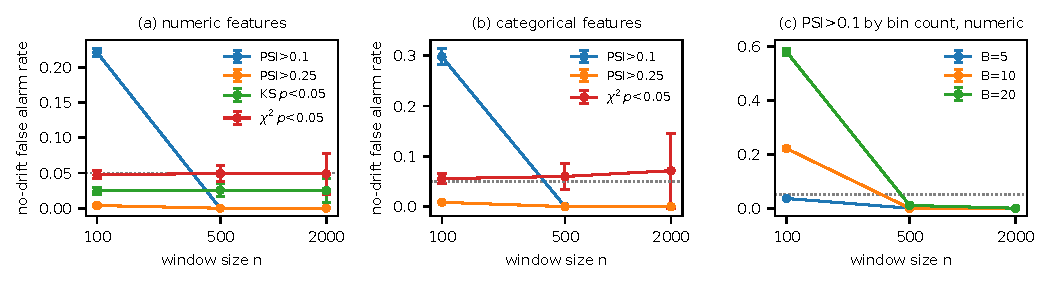
\includegraphics[width=\textwidth]{figures/fig_null_fpr.pdf}
\caption{No-drift false alarm rate of threshold rules versus window size (mean and standard deviation over five seeds). (a) numeric and (b) categorical features; (c) PSI${}>0.1$ with $B\in\{5,10,20\}$ bins. The dotted line marks 0.05.}
\label{fig:null}
\end{figure*}

\section{Evaluation}
\label{sec:eval}

\subsection{Setup}
\label{sec:eval-setup}

\subsubsection{Data}
We use three public OpenML datasets~\cite{vanschoren2014,feurer2019}: adult~\cite{adult}, bank-marketing~\cite{moro2014}, and electricity (Elec2)~\cite{elec2}. From them we monitor 18 numeric and 9 categorical features (Table~\ref{tab:tpr} lists the drift types). Of the numeric features, 13 are discrete (integer-valued, or on a regular grid with few levels) and 5 are continuous. A missing categorical value is treated as a category of its own. URLs, licenses, retrieval dates, and SHA-256 hashes are recorded in \texttt{data/SOURCES.md}.

\begin{table*}[!t]
\caption{TPR at a calibrated per-window false alarm rate of 0.05, averaged over magnitudes $\{0.05,0.1,0.2,0.4\}$ (mean$\pm$std over five seeds; 18 numeric or 9 categorical features). Drift is simulated.}
\label{tab:tpr}
\centering
\footnotesize
\begin{tabular}{llccccc}
\toprule
Drift type & $n$ & PSI & KL & $\chi^2$ & KS & W1 \\
\midrule
mean shift & 100 & 0.74$\pm$0.01 & 0.74$\pm$0.01 & 0.74$\pm$0.01 & 0.74$\pm$0.01 & 0.48$\pm$0.03 \\
mean shift & 500 & 0.86$\pm$0.02 & 0.86$\pm$0.02 & 0.86$\pm$0.02 & 0.86$\pm$0.01 & 0.69$\pm$0.02 \\
mean shift & 2000 & 0.92$\pm$0.02 & 0.92$\pm$0.02 & 0.92$\pm$0.02 & 0.92$\pm$0.01 & 0.84$\pm$0.03 \\
scale change & 100 & 0.29$\pm$0.02 & 0.29$\pm$0.02 & 0.30$\pm$0.02 & 0.25$\pm$0.01 & 0.27$\pm$0.01 \\
scale change & 500 & 0.54$\pm$0.02 & 0.54$\pm$0.02 & 0.54$\pm$0.02 & 0.53$\pm$0.03 & 0.47$\pm$0.02 \\
scale change & 2000 & 0.69$\pm$0.03 & 0.69$\pm$0.03 & 0.69$\pm$0.03 & 0.71$\pm$0.03 & 0.63$\pm$0.01 \\
selection shift & 100 & 0.27$\pm$0.01 & 0.28$\pm$0.01 & 0.28$\pm$0.01 & 0.35$\pm$0.01 & 0.35$\pm$0.01 \\
selection shift & 500 & 0.50$\pm$0.02 & 0.50$\pm$0.02 & 0.50$\pm$0.02 & 0.58$\pm$0.02 & 0.56$\pm$0.01 \\
selection shift & 2000 & 0.66$\pm$0.03 & 0.66$\pm$0.03 & 0.66$\pm$0.03 & 0.73$\pm$0.03 & 0.71$\pm$0.03 \\
frequency shift (cat.) & 100 & 0.41$\pm$0.03 & 0.46$\pm$0.03 & 0.46$\pm$0.02 & n/a & n/a \\
frequency shift (cat.) & 500 & 0.60$\pm$0.04 & 0.63$\pm$0.03 & 0.61$\pm$0.03 & n/a & n/a \\
frequency shift (cat.) & 2000 & 0.73$\pm$0.04 & 0.75$\pm$0.04 & 0.72$\pm$0.04 & n/a & n/a \\
\bottomrule
\end{tabular}
\end{table*}

\begin{figure*}[!t]
\centering
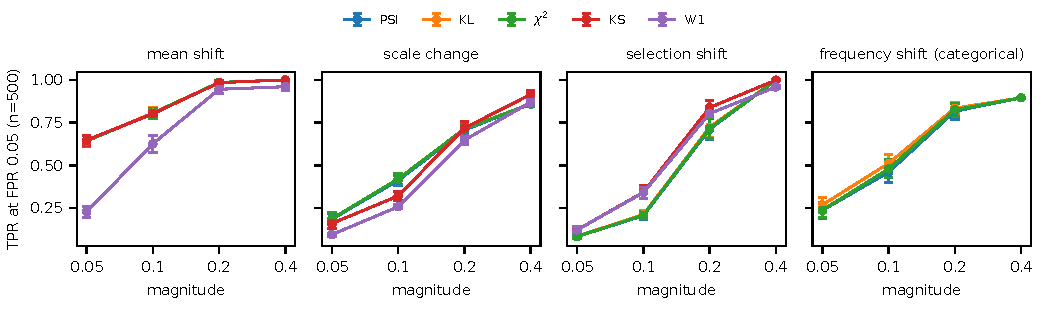
\includegraphics[width=\textwidth]{figures/fig_tpr_calibrated.pdf}
\caption{TPR at a calibrated false alarm rate of 0.05 versus drift magnitude for $n=500$ (mean and standard deviation over five seeds). Drift is simulated.}
\label{fig:tpr}
\end{figure*}

\subsubsection{Detector benchmark (RQ1, RQ2)}
For each feature and seed, we split the rows at random into a reference half and a test half. The reference sample holds $m=1000$ rows, and windows of size $n\in\{100,500,2000\}$ are drawn with replacement from the test half. Per feature, window size, and seed we draw 200 no-drift windows for calibration, 200 independent no-drift windows for evaluation, and 100 windows for each drift configuration. Numeric features get three drift types. A mean shift adds $\delta$ reference standard deviations. A scale change multiplies deviations from the reference median by $1+\delta$. A selection shift samples rows with probability proportional to $\exp(\beta z)$, where $z$ is the rank-based normal score of the value. Categorical features get a frequency shift toward uniform, $p'=(1-\delta)p+\delta/K$. Magnitudes are $\delta,\beta\in\{0.05,0.1,0.2,0.4\}$. After a shift, values of discrete features are rounded back to their grid with unbiased stochastic rounding. All of this drift is simulated.

\subsubsection{Streaming delay (RQ3)}
For each numeric feature we build 20 streams of batches with $n=200$. Each stream starts with 10 no-drift batches, after which a mean shift ramps linearly from zero to 0.5 standard deviations over 30 batches. Per-batch thresholds are calibrated at $\phi=0.01$ on 500 no-drift batches, and the delay is the index of the first alarm after onset. For compute time we take the median of 200 calls per detector on one Apple M3 laptop, with reference summaries precomputed.

\subsubsection{Portfolio simulation (RQ4)}
Each model has $F=20$ Gaussian features, a reference of $m=1000$, and one daily window of $n=200$ per feature over $T=30$ days. Of the models, 10\% drift. A drifting model shifts the means of one to five features by $|\delta|\sim U(0.1,0.5)$ standard deviations with random sign, starting on an onset day drawn uniformly in $[5,20]$. Every test is a two-sample KS test. We run $N\in\{10,100,1000\}$, and at $N=1000$ we add four breakpoint scenarios: within-model equicorrelation $\rho=0.6$, 10\% of $p$-values missing (handled by exclusion or by $p=1$), and window sizes 100 and 500. This drift is simulated as well.

\subsubsection{Input versus performance alarms (RQ5)}
Elec2 holds half-hourly records in temporal order, which we group into weekly batches of 336 rows. Each of five runs trains a random forest~\cite{breiman2001,pedregosa2011} with 100 trees on six weeks of data starting at week 52, 60, 68, 76, or 84. The run validates on the next two weeks and then monitors the following 40 weeks. Before row 17377, the Victoria price, Victoria demand, and transfer columns hold a constant fill value left by the data pipeline, so every training window starts after it. The performance alarm is a one-sided two-proportion $z$-test of the weekly error against the validation error at $\alpha=0.05$. The input alarm applies the KS test to five features (prices, demands, transfer) against the eight training weeks, with BH at $q=0.05$ across features. We also report the rule ``any feature PSI${}>0.25$''.

\subsubsection{Statistics}
Each configuration runs with seeds 0 to 4. We report the mean and standard deviation over seeds, and $t$-based 95\% confidence intervals for the hypothesis decisions. Every rate comes with its denominator, in the text or in a table.

\subsection{RQ1: Rule-of-thumb thresholds on no-drift windows}
\label{sec:res-null}

Table~\ref{tab:null} and Fig.~\ref{fig:null} show how often common rules fire on windows that contain no drift. The rule ``PSI${}>0.1$'' fired on 22.1\% of numeric no-drift windows at $n=100$ (3982 of 18000 windows) and on none at $n=500$ or $n=2000$. On categorical features it fired on 29.8\% at $n=100$ (2684 of 9000). So one PSI threshold means a different false alarm rate at each window size. H2 is supported: the mean gap between $n=100$ and $n=2000$ was 0.221 (95\% CI 0.214 to 0.229), above the registered bound of 0.10. The number of bins moves the rate again (Fig.~\ref{fig:null}c). At $n=100$, PSI${}>0.1$ fired on 3.6\% of windows with $B=5$ and on 58.0\% with $B=20$. The KS test at $p<0.05$ fired on 2.5\% of numeric windows at $n=100$ (442 of 18000), which is below its nominal level; 13 of the 18 numeric features are discrete, and the KS test is conservative with ties. On numeric features the chi-square test stayed near its nominal level (4.8\% at $n=100$). On categorical features at $n=2000$ it fired on 7.1\% of windows (643 of 9000), and the spread across seeds was large (std 0.075).

\begin{table}[!t]
\caption{False alarms of rule-of-thumb thresholds on no-drift windows (alarms/windows, pooled over features and five seeds).}
\label{tab:null}
\centering
\scriptsize
\setlength{\tabcolsep}{3pt}
\begin{tabular}{llrrr}
\toprule
Features & Rule & $n=100$ & $n=500$ & $n=2000$ \\
\midrule
numeric & PSI$>$0.1 & 3982/18000 & 0/18000 & 0/18000 \\
numeric & PSI$>$0.25 & 71/18000 & 0/18000 & 0/18000 \\
numeric & KS $p$$<$0.05 & 442/18000 & 465/18000 & 452/18000 \\
numeric & $\chi^2$ $p$$<$0.05 & 857/18000 & 887/18000 & 880/18000 \\
categorical & PSI$>$0.1 & 2684/9000 & 3/9000 & 0/9000 \\
categorical & PSI$>$0.25 & 78/9000 & 0/9000 & 0/9000 \\
categorical & $\chi^2$ $p$$<$0.05 & 500/9000 & 540/9000 & 643/9000 \\
\bottomrule
\end{tabular}
\end{table}

\subsection{RQ2: Detector sensitivity at a calibrated false alarm rate}
\label{sec:res-detectors}

Calibration kept the measured false alarm rate close to its target. Over all detectors, feature types, and window sizes, the rate on the separate evaluation windows ranged from 0.0455 to 0.0563. Table~\ref{tab:tpr} gives the true positive rate (TPR) averaged over the four magnitudes, and Fig.~\ref{fig:tpr} shows it per magnitude at $n=500$.

No detector dominated. At $n=500$, the binned detectors and KS detected mean shifts at a TPR of 0.858 to 0.859, while W1 reached 0.690, and on the 5 continuous features W1 fell to 0.603. For scale changes the binned detectors reached 0.540 to 0.545, KS 0.528, and W1 0.467. Splitting by feature type shows that part of this ranking comes from discreteness. On continuous features the binned detectors led for scale changes (0.636 to 0.643 against 0.513 for KS). On discrete features KS led (0.534 against 0.503 to 0.507). For selection shifts KS led (0.575), followed by W1 (0.556) and the binned detectors (0.499 to 0.504). On categorical features KL, chi-square, and PSI reached 0.627, 0.609, and 0.602, and these differences are smaller than one seed standard deviation. TPR grew with the window size for every detector; for selection shifts, KS rose from 0.346 at $n=100$ to 0.735 at $n=2000$. W1 divides by the reference standard deviation, so outliers in heavy-tailed features may widen its null distribution. We did not test this explanation.

The PSI bin count trades sensitivity on one drift type for sensitivity on another. At $n=500$ and a scale change of 0.1, $B=20$ reached a TPR of 0.461, against 0.411 for $B=10$ and 0.231 for $B=5$. For a selection shift of 0.2 the order reversed: 0.764 for $B=5$, 0.712 for $B=10$, and 0.603 for $B=20$.

\subsection{RQ3: Detection delay, compute cost}
\label{sec:res-delay}

Table~\ref{tab:delay} reports the streaming ramp. With per-batch thresholds at a false alarm rate of 0.01, each detector raised between 0.093 and 0.108 false alarms in the 10 pre-change batches of a stream, which is what the calibration implies. PSI, KL, chi-square, and KS detected every stream, on average after 4.66 to 4.75 batches, when the shift had reached about 0.078 to 0.079 standard deviations. W1 was slower. It detected 0.977 of the streams within 30 batches and needed 8.98 batches on average, by which point the shift was 0.150 standard deviations. Table~\ref{tab:timing} gives the cost of one call. The binned detectors were the cheapest at both sizes and SciPy's KS test the most expensive. Because our KS and W1 share one sort, computing both statistics cost less than SciPy's KS test alone.

\begin{table}[!t]
\caption{Streaming mean-shift ramp ($n=200$, per-batch false alarm rate 0.01): false alarms in the 10 pre-change batches per stream, fraction of streams detected within 30 batches, mean delay among detected streams, and the shift magnitude reached at the mean delay (mean$\pm$std over five seeds).}
\label{tab:delay}
\centering
\scriptsize
\setlength{\tabcolsep}{3pt}
\begin{tabular}{lrrrr}
\toprule
Detector & Pre-change FA & Detected & Delay (batches) & $\delta$ at alarm \\
\midrule
PSI & 0.102$\pm$0.012 & 1.000$\pm$0.000 & 4.72$\pm$0.24 & 0.079$\pm$0.004 \\
KL & 0.102$\pm$0.015 & 1.000$\pm$0.000 & 4.70$\pm$0.22 & 0.078$\pm$0.004 \\
$\chi^2$ & 0.099$\pm$0.011 & 1.000$\pm$0.000 & 4.75$\pm$0.23 & 0.079$\pm$0.004 \\
KS & 0.093$\pm$0.009 & 1.000$\pm$0.000 & 4.66$\pm$0.27 & 0.078$\pm$0.004 \\
W1 & 0.108$\pm$0.019 & 0.977$\pm$0.022 & 8.98$\pm$0.46 & 0.150$\pm$0.008 \\
\bottomrule
\end{tabular}
\end{table}

\begin{table}[!t]
\caption{Median time per call in microseconds on one Apple M3 laptop shared with other jobs (reference summary precomputed; 200 calls).}
\label{tab:timing}
\centering
\footnotesize
\begin{tabular}{lrr}
\toprule
Call & $n=m=1000$ & $n=m=10000$ \\
\midrule
binned PSI+KL+$\chi^2$ (ours) & 41 & 128 \\
KS (SciPy, asymptotic) & 310 & 4863 \\
W1 (SciPy) & 91 & 2481 \\
KS+W1 (ours, shared sort) & 94 & 1368 \\
\bottomrule
\end{tabular}
\end{table}

\begin{table*}[!t]
\caption{Simulated portfolio, base scenario ($F=20$, $n=200$, $m=1000$, 30 days; mean$\pm$std over five seeds). FA/day: rejected tests on non-drifted features per day. Model FA/day: alarmed models without any drifted feature. FDP: false discovery proportion per day. Recall@3d: drift events detected within three days of onset. Delay: mean days to detection among detected events.}
\label{tab:portfolio}
\centering
\footnotesize
\begin{tabular}{rlrrrrr}
\toprule
$N$ & Policy & FA/day & Model FA/day & FDP & Recall@3d & Delay (d) \\
\midrule
10 & per-test & 10.00$\pm$0.37 & 6.15$\pm$0.06 & 0.907$\pm$0.042 & 1.00$\pm$0.00 & 0.00$\pm$0.00 \\
10 & Bonferroni & 0.10$\pm$0.07 & 0.09$\pm$0.07 & 0.076$\pm$0.051 & 0.80$\pm$0.45 & 0.80$\pm$1.79 \\
10 & BH & 0.16$\pm$0.11 & 0.14$\pm$0.12 & 0.095$\pm$0.053 & 0.80$\pm$0.45 & 0.80$\pm$1.79 \\
10 & hierarchical & 0.13$\pm$0.08 & 0.12$\pm$0.08 & 0.089$\pm$0.054 & 0.80$\pm$0.45 & 0.80$\pm$1.79 \\
\midrule
100 & per-test & 96.27$\pm$2.70 & 59.29$\pm$1.19 & 0.877$\pm$0.021 & 0.98$\pm$0.04 & 0.06$\pm$0.13 \\
100 & Bonferroni & 0.02$\pm$0.03 & 0.02$\pm$0.03 & 0.008$\pm$0.016 & 0.78$\pm$0.08 & 0.80$\pm$0.42 \\
100 & BH & 0.44$\pm$0.13 & 0.41$\pm$0.10 & 0.046$\pm$0.034 & 0.88$\pm$0.08 & 0.54$\pm$0.78 \\
100 & hierarchical & 0.21$\pm$0.12 & 0.20$\pm$0.11 & 0.040$\pm$0.043 & 0.86$\pm$0.05 & 0.76$\pm$0.81 \\
\midrule
1000 & per-test & 956.43$\pm$7.07 & 592.39$\pm$2.59 & 0.876$\pm$0.006 & 0.97$\pm$0.01 & 0.14$\pm$0.05 \\
1000 & Bonferroni & 0.06$\pm$0.04 & 0.06$\pm$0.04 & 0.002$\pm$0.002 & 0.69$\pm$0.03 & 1.47$\pm$0.31 \\
1000 & BH & 4.19$\pm$0.34 & 3.95$\pm$0.35 & 0.041$\pm$0.004 & 0.84$\pm$0.01 & 1.01$\pm$0.14 \\
1000 & hierarchical & 2.28$\pm$0.27 & 2.26$\pm$0.28 & 0.040$\pm$0.006 & 0.82$\pm$0.01 & 1.06$\pm$0.17 \\
\bottomrule
\end{tabular}
\end{table*}

\subsection{RQ4: Alarm policies at portfolio scale}
\label{sec:res-portfolio}

\begin{figure}[!t]
\centering
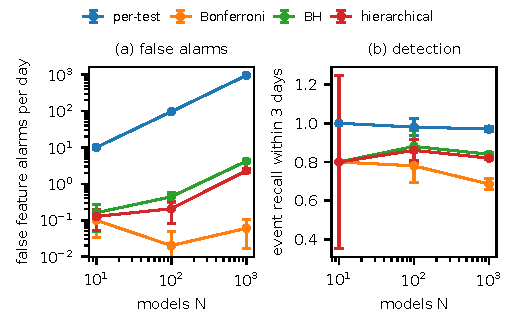
\includegraphics[width=\columnwidth]{figures/fig_portfolio.pdf}
\caption{Simulated portfolio: (a) false feature alarms per day (log scale; zero shown at 0.01) and (b) three-day event recall versus the number of models (mean and standard deviation over five seeds).}
\label{fig:portfolio}
\end{figure}

Table~\ref{tab:portfolio} and Fig.~\ref{fig:portfolio} summarize the simulated portfolio. Per-test thresholds produced 10.0, 96.3, and 956.4 false feature alarms per day for $N=10$, 100, and 1000. That is linear in the number of tests, as expected. At $N=1000$, 592.4 models without any drifted feature raised an alarm each day, and the false discovery proportion of per-test alarms was 0.876. At the same scale BH produced 4.19 false feature alarms per day, with a false discovery proportion of 0.041.

The price of this reduction is detection speed. At $N=1000$, per-test thresholds detected 0.970 of the drift events within three days. BH detected 0.840, the hierarchical policy 0.820, and Bonferroni 0.686. Over the whole 30-day horizon, BH detected 0.942 of the events with a mean delay of 1.01 days. The preregistered endpoints of \eqref{eq:endpoints} were $R_{\mathrm{FA}}=0.9956$ (95\% CI 0.9952 to 0.9961) and $RR=0.866$ (95\% CI 0.850 to 0.883). Both lower bounds clear their thresholds, so H1 is supported for this configuration. The hierarchical policy produced about half the false alarms of BH (2.28 per day) for a small loss in recall, and each of its alarms names one feature of the alarmed model.

Table~\ref{tab:scenarios} tests the breakpoints. Within-model correlation ($\rho=0.6$) left the BH false discovery proportion at 0.046 and its three-day recall at 0.836. It did concentrate the per-test false alarms in fewer models (409.6 alarmed models per day instead of 592.4). With 10\% of the $p$-values missing, 2000.4 tests per day were unknown, and excluding them from the family or setting them to one gave nearly the same recall (0.826 and 0.822). The BH false discovery proportion rose to 0.062 (95\% CI 0.026 to 0.097); that interval contains the nominal 0.05. Window size is the breakpoint that matters most. With $n=100$, BH detected only 0.580 of the events within three days against 0.964 for per-test thresholds, so the 80\% retention that H1 requires fails at that window size. With $n=500$, BH reached 0.946 against 0.994.

\begin{table}[!t]
\caption{Breakpoint scenarios at $N=1000$ (mean$\pm$std over five seeds; simulated drift).}
\label{tab:scenarios}
\centering
\scriptsize
\setlength{\tabcolsep}{3pt}
\begin{tabular}{llrrr}
\toprule
Scenario & Policy & FA/day & FDP & Recall@3d \\
\midrule
independent, $n=200$ & per-test & 956.4$\pm$7.1 & 0.876$\pm$0.006 & 0.97$\pm$0.01 \\
independent, $n=200$ & BH & 4.2$\pm$0.3 & 0.041$\pm$0.004 & 0.84$\pm$0.01 \\
independent, $n=200$ & hierarchical & 2.3$\pm$0.3 & 0.040$\pm$0.006 & 0.82$\pm$0.01 \\
$\rho=0.6$ & per-test & 955.3$\pm$15.1 & 0.879$\pm$0.005 & 0.99$\pm$0.01 \\
$\rho=0.6$ & BH & 4.4$\pm$0.7 & 0.046$\pm$0.009 & 0.84$\pm$0.03 \\
$\rho=0.6$ & hierarchical & 2.1$\pm$0.2 & 0.039$\pm$0.007 & 0.82$\pm$0.04 \\
10\% missing, exclude & per-test & 862.8$\pm$2.7 & 0.883$\pm$0.003 & 0.98$\pm$0.01 \\
10\% missing, exclude & BH & 3.4$\pm$0.1 & 0.062$\pm$0.029 & 0.83$\pm$0.04 \\
10\% missing, exclude & hierarchical & 2.1$\pm$0.2 & 0.062$\pm$0.030 & 0.81$\pm$0.05 \\
10\% missing, $p{=}1$ & per-test & 862.8$\pm$2.7 & 0.883$\pm$0.003 & 0.98$\pm$0.01 \\
10\% missing, $p{=}1$ & BH & 3.1$\pm$0.1 & 0.057$\pm$0.029 & 0.82$\pm$0.04 \\
10\% missing, $p{=}1$ & hierarchical & 1.9$\pm$0.2 & 0.057$\pm$0.030 & 0.81$\pm$0.05 \\
$n=100$ & per-test & 981.0$\pm$5.0 & 0.902$\pm$0.005 & 0.96$\pm$0.02 \\
$n=100$ & BH & 1.5$\pm$0.3 & 0.064$\pm$0.014 & 0.58$\pm$0.08 \\
$n=100$ & hierarchical & 1.2$\pm$0.2 & 0.062$\pm$0.015 & 0.56$\pm$0.07 \\
$n=500$ & per-test & 1014.1$\pm$5.4 & 0.870$\pm$0.005 & 0.99$\pm$0.01 \\
$n=500$ & BH & 5.8$\pm$0.5 & 0.052$\pm$0.020 & 0.95$\pm$0.02 \\
$n=500$ & hierarchical & 2.5$\pm$0.3 & 0.053$\pm$0.018 & 0.93$\pm$0.03 \\
\bottomrule
\end{tabular}
\end{table}

\subsection{RQ5: Input drift versus performance on Elec2}
\label{sec:res-elec}

Table~\ref{tab:elec} and Fig.~\ref{fig:elec} report the Elec2 study. The input-drift alarm (KS with BH across five features) fired in all 200 monitored weeks of the five runs. So did the rule ``any feature PSI${}>0.25$''. Performance alarms fired in 138 of the 200 weeks, and the per-run rate ranged from 0.30 to 1.00. Read as a predictor of performance alarms, the input alarm had a precision of 138/200 and a recall of 138/138. The input series never changed, so Cohen's $\kappa$ was 0 in the four runs where the performance series varied. In the run starting at week 68 both series were constant and $\kappa$ was undefined. H3 is supported by its registered rule, but the result is degenerate. With 336 rows per week, the tests reject an unchanged input distribution in every week of this non-stationary stream. The continuous statistics carried only weak information. Across runs, Spearman's correlation between the weekly maximum PSI and the accuracy drop was 0.258 (std 0.156); for the maximum KS statistic it was 0.313 (std 0.122). No week lacked labels, so the unknown branch of the performance test was not exercised.

\begin{table}[!t]
\caption{Elec2 weekly monitoring over 40 weeks per run: validation accuracy, weeks with a performance alarm, weeks with an input-drift alarm (KS with BH across five features), Cohen's $\kappa$ between the two alarm series, and Spearman's $\rho_s$ between the maximum PSI and the accuracy drop.}
\label{tab:elec}
\centering
\scriptsize
\setlength{\tabcolsep}{3pt}
\begin{tabular}{rrrrrr}
\toprule
Start wk & Val. acc. & Perf. alarms & Input alarms & $\kappa$ & $\rho_s$ \\
\midrule
52 & 0.838 & 38/40 & 40/40 & 0.000 & 0.456 \\
60 & 0.713 & 12/40 & 40/40 & 0.000 & 0.256 \\
68 & 0.854 & 40/40 & 40/40 & n/a & 0.094 \\
76 & 0.684 & 18/40 & 40/40 & 0.000 & 0.365 \\
84 & 0.780 & 30/40 & 40/40 & 0.000 & 0.118 \\
\bottomrule
\end{tabular}
\end{table}

\begin{figure}[!t]
\centering
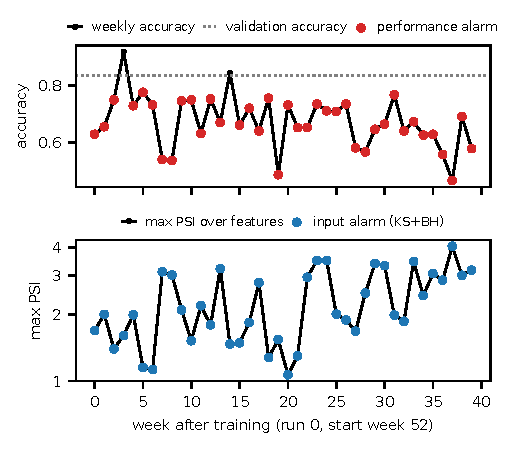
\includegraphics[width=\columnwidth]{figures/fig_electricity.pdf}
\caption{Elec2, run 0: weekly accuracy with performance alarms (top) and maximum PSI over the five monitored features with input-drift alarms (bottom).}
\label{fig:elec}
\end{figure}

\section{Threats to Validity}
\label{sec:threats}

\subsection{Simulated drift (internal and construct validity)}

The detector benchmark injects four synthetic perturbations into resampled real values, and the portfolio study uses Gaussian features with sudden, persistent mean shifts. Production drift can be gradual, seasonal, or recurring, or it can sit in the joint distribution while the marginals stay stable~\cite{webb2016}. The ranking of detectors depends on these choices. Additive offsets, for example, are easy to detect on zero-inflated features, which is why we split the results into discrete and continuous features. The portfolio result for BH depends on the effect-size range of the injected shifts and on the window size.

\subsection{Exchangeable null windows}

No-drift windows are drawn at random from a held-out half of each dataset, so they are exchangeable with the reference. Real streams are autocorrelated and seasonal. On real streams, rule-of-thumb and calibrated false alarm rates will be higher than our null estimates, as the Elec2 study suggests.

\subsection{Untested breakpoints}

We did not test (i) drift events shared by many models through a common upstream source, which correlates the tests across models; (ii) adversarial or deliberately crafted inputs; (iii) multivariate shift with stable marginals, which univariate detectors cannot see by construction; (iv) delayed or partial label feeds, which Algorithm~\ref{alg:cycle} handles by abstaining but whose delay cost we did not measure; (v) monitoring periods shorter than one day or more than 20000 tests per period; and (vi) features with heavy missingness beyond the 10\% scenario.

\subsection{Baselines not run}

Sequential detectors (CUSUM\slash Page-Hinkley~\cite{page1954}, DDM~\cite{gama2004}, ADWIN~\cite{bifet2007}), online FDR rules~\cite{javanmard2018,ramdas2017online}, adaptive FDR with an estimated null proportion~\cite{storey2002}, kernel and classifier two-sample tests~\cite{gretton2008,rabanser2019}, and label-free performance estimators~\cite{garg2022,nannyml} were not run. Version 1 reported production case studies. No production logs were available to this revision, so those studies could not be reproduced and were removed.

\subsection{Measurement choices}

False alarms per day and three-day recall are proxies for operator cost and for the harm of late detection, and both ignore severity. The Elec2 performance test assumes independent errors within a week; autocorrelated errors would inflate its alarm rate. Timing was measured on one laptop that other jobs shared during the run, so the absolute times are upper bounds for that machine. Ratios between detectors are more stable than absolute values.

\subsection{Claims outside the evaluation}

We make no claims about the full three-tier architecture, Kubernetes deployment, retraining automation, regulatory compliance, or business impact, since none of them was evaluated. The scale at which per-test thresholds become unusable depends on the alarm budget $\beta$ in \eqref{eq:objective}, and each organization has to set that budget.

\section{Conclusion}
\label{sec:conclusion}

This revision keeps the monitoring design of version 1 and puts preregistered measurements where its unmeasured numbers were. Four findings hold under the stated conditions.

Rule-of-thumb PSI thresholds do not fix a false alarm rate. The rule PSI${}>0.1$ fired on 22.1\% of no-drift numeric windows of size 100 and on none of size 2000, so thresholds should be calibrated per feature and window size. At an equal false alarm rate, no detector dominated: the binned detectors and KS led on mean shifts, KS led on selection shifts, and W1 trailed on mean shifts and on gradual drift.

In a simulated portfolio of 1000 models, per-test thresholds produced 956.4 false feature alarms per day. BH produced 4.19 and kept 86.6\% of the per-test three-day recall, so the preregistered hypothesis H1 was supported. That support depends on the window size. With 100 rows per window, recall retention fell well below the registered bound.

On Elec2, weekly input-drift tests alarmed in every monitored week, while performance alarms fired in 138 of 200 weeks. Input drift can tell an operator which model to look at first. It cannot replace labelled evaluation. Future work should measure online FDR rules and sequential detectors on the same portfolio workload and test correlated drift across models.

\section*{Data and Code Availability}
The Zenodo record of this version holds the paper source, the experiment code, the cached OpenML data with its provenance in \texttt{data/SOURCES.md}, the logged results, the unit tests, and \texttt{preregistration.json}. Running \texttt{python code/run\_all.py} downloads the data or reuses the cached copy, runs every experiment with seeds 0 to 4, writes \texttt{results/}, and regenerates all figures and tables. The unit tests run with \texttt{python -m pytest tests}.

\appendices
\section{Disposition of Version-1 Claims}
\label{app:v1}

Table~\ref{tab:v1} lists the quantitative claims of version 1 and what this revision did with each. We do not repeat the numbers of removed claims, because no source or log supports them.

\begin{table}[!t]
\caption{Version-1 claims and their treatment in version 2.}
\label{tab:v1}
\centering
\footnotesize
\setlength{\tabcolsep}{3pt}
\renewcommand{\arraystretch}{1.15}
\begin{tabular}{>{\raggedright\arraybackslash}p{4.6cm}>{\raggedright\arraybackslash}p{3.3cm}}
\toprule
Version-1 claim & Version-2 action \\
\midrule
Industry prevalence, detection-time, and cost statistics without sources & removed \\
Three anecdotal failure cases with dollar figures & removed \\
Fraud, healthcare, and e-commerce case studies (portfolio size, detection-time and alert reductions, significance tests, rater agreement) & removed; no data or logs exist \\
Detector sensitivity and specificity table & replaced by the calibrated benchmark (Section~\ref{sec:res-detectors}) \\
Detector compute times without hardware or sample size & replaced by measured times (Table~\ref{tab:timing}) \\
Universal PSI interpretation bands & reframed as window-size dependent (Section~\ref{sec:res-null}) \\
Tier-scoring weights and tier-assignment ablation & removed; not measured \\
Detection latency and compute scaling at portfolio size & replaced by the portfolio simulation (Section~\ref{sec:res-portfolio}) \\
Three-tier architecture, alert levels, retraining flow & kept as a design (Table~\ref{tab:tiers}), not evaluated \\
Regulatory compliance mapping & removed \\
\bottomrule
\end{tabular}
\end{table}

\section*{Acknowledgment}
Generative AI was used to prepare this revision. Large language models (GitHub Copilot with Anthropic Claude) critiqued the version-1 methodology, generated the experiment code, and drafted and edited the text. In a final pass, the same model edited the wording for style. Every reported number, table, and figure was produced by code from the logged experiment results; none was written by a language model.

\IEEEtriggeratref{31}
\bibliographystyle{IEEEtran}
\bibliography{references}

\end{document}
